\chapter{Signal Modeling\label{chap:sigmod}}

\section{Introduction}

To build tools to analyse and synthesize signals some structure must be imposed
on the signals. The structures chosen can reflect something about the behaviour
of these signals as observed in the field, as we will see with sinusoidal
models. Other structures are chosen phenomenologically --- we do not really know
the underlying mechanism behind the production of these signals, but a
particular structure is chosen for its mathematical or conceptual convenience,
such as is the case when we consider higher-order models for sinusoidal phase
and amplitude.

We begin the chapter with what could be seen as a mathematical analog of the
musical score: time-frequency representations. Through this we will justify the
adoption of a sinusoidal model for musical signals. Finding this inadequate to
describe the signals of interest with sufficient quality, the sinusoidal model
is generalized to incorporate modulations in frequency and amplitude. A
technique is described to estimate the parameters of these more complex models
which requires windows that are everywhere differentiable --- we design a new
window having desirable properties close to those of well-known optimal windows,
but that is everywhere differentiable.

\section{Time-Frequency Representations \label{sec:timefreqrep}}

As most musical instruments are resonating media, and excited resonating media
are well described as linear time-invariant (LTI) auto-regressive (AR)
structures, many popular models of musical audio are some variation of this
description \cite{fletcher2012physics}. Strictly speaking, incorporating
moving-average (MA) structures into a model of musical signals could improve its
quality, but such a model would preclude the sum-of-sinusoids model adopted
later in this thesis.

An LTI auto-regressive structure is a signal that can be described using the
following \textit{difference equation}:

\[
    x(n) = \sum_{k=1}^{K} a_k x(n-k) + b_0 v(n)
\]

Here $x$ is the output of the system (what is heard or measured) and $v$ is the
input. $K$ is the order of the model. Both are general functions of time which,
in the case of properly sampled digital audio, can be considered at discrete
times $n \in \mathbb{Z}$ without any loss of information
\cite[ch.~2]{crochiere1983multi}.  $a_k,b_0 \in \mathbb{C}$ and are constants.
Casually you can think of the output of the system at
time $n$ as being a linear combination of past outputs, plus some of the scaled
input.

AR structures are excited in various ways: some are bowed, others struck, etc.
To characterize the above structure we excite it with a simple signal, the
\textit{Kronecker delta}

\[
    \delta(n) = \begin{cases}
        1 & n=0\\
        0 & \text{otherwise}
    \end{cases}
\]

This Kronecker delta input will yield its \textit{impulse
response} from which we can derive many properties of the AR structure.

As an example take the case where $K=1$ and $a_1 = r \exp(j\omega)$, 
$r, \omega \in \mathbb{R}$, $|r|<1$. Then the difference equation is
\[
    x(n) = r \exp(j\omega) x(n-1) + v(n)
\]
Exciting this with the Kronecker delta we get
\[
    \begin{array}{c}
        x(0) = 1 \\
        x(1) = r \exp(j\omega) \\
        x(n) = r^n \exp(j\omega n)
    \end{array}
\]
which is a complex exponential starting at $n=0$ and periodic in
$n_T=\frac{2\pi}{\omega}$ multiplied by the real-valued
exponential $r^n$. In other words, the output is a damped sinusoid. From this
it is not hard to see that if we can estimate the coefficients $a_k$, we can
then know the frequencies, amplitudes and damping factors of the sinusoids that
are output when this structure is excited by an impulse (the Kronecker delta).
This principle is presented as a motivation for the following techniques and is
not pursued here. The interested reader is referred to \cite{makhoul1975linear}
for more information.

An alternative method for determining the frequencies and amplitudes of
sinusoids in mixture is to take the inner product of the signal with a complex
exponential of known frequency

\[
    X(\omega) = \sum_{n=-\infty}^{\infty} x(n) \exp(-j \omega n)
\]

The function $X(\omega)$ will be large if $x(n)$ contains a complex exponential of
frequency $\omega$ and small if it does not, effectively indicating which
sinusoidal functions are present in the signal. This transformation of a signal
as a function of time $n$ into one as a function of frequency $\omega$ is known
as the \textit{Discrete-time Fourier Transform} (DTFT). 

To create a variety of pitches and timbres, typically the media of musical
instruments are not static, but vary in time. That means the sets of sinusoids
describing the state of the media and its excitation also change in time. To
account for this we consider many small intervals of signal where we assume its
characteristics are roughly static. We can then piece these time-intervals
together afterwards to get a description of the signal in both time and
frequency. To do this, we multiply the signal by a window $w$ which makes the signal
0 outside of the interval of interest. We then test what sinusoids with
frequencies $\omega$ are present at different times $\tau$, giving a function of
two variables

\begin{equation}
    \label{eq:dtstftdef}
    X(\tau,\omega) = \sum_{n=-\infty}^{\infty} x(n) w(n - \tau) \exp(-j \omega n)
\end{equation}
This transformation of a signal of time $n$ into one of time $\tau$ and
frequency $\omega$ is known as the \textit{Discrete-time Short-time Fourier
Transform} (DTSTFT).

One further point about the window should be discussed. The Fourier transform of
the product of two functions, like we have in Equation~\ref{eq:dtstftdef}, is
equal to the convolution of the Fourier transform of each function separately.
If we denote the Fourier transform operator as $\mathcal{F}$, for functions $g$
and $f$ we have
\[
    \mathcal{F}(gf) = \mathcal{F}(g)\ast\mathcal{F}(f)
\]
where $\ast$ is the convolution operator. The value $X(\tau,\omega)$, which will
be a complex number, can be seen
as describing the amplitude and phase of a sinusoid at that frequency and time.
If the Fourier transform of the window function is not purely real its imaginary
part will offset the phase of this sinusoid. It is usually simpler to avoid this
complication. The Fourier transform of a real even function
\[
    f(n) = f(-n), f(n) \in \mathbb{R}
\]
is real, so we choose windows with this property. See
\cite[p.~52]{harris1978use} for a concrete illustration of this.

\section{Polynomial Phase Models\label{sec:polynomphasemodel}}

The DTFT and DTSTFT are very useful because they are invertible
\cite{portnoff1976implementation}%
\footnote{Provided proper sampling in time and frequency.}
and fast algorithms exist for their 
computation by digital computer \cite{van1992computational}. If the presence of
a sinusoid is determined, e.g., by finding $\tau^{\ast}$ and $\omega^{\ast}$ such that
$X$ is maximized, that signal can be removed or altered easily.

One drawback of these transforms is they only project onto sinusoidal functions
of linear phase, i.e., functions of constant frequency. In general, musical
signals are not linear combinations of sinusoids of constant frequency
(consider, for example, vibrato). We could decide to project onto a different
family of functions and considerable effort has been devoted to finding
alternatives (see \cite{kereliuk2011sparse} for a review). In the case of
musical signals, however, we have some prior information about the mechanics of
the their production and can make certain assumptions about the underlying
functions.

\subsection{Sinusoidal Representations\label{sec:mqfmfromphase}} Many musical
acoustic signals are quasi-harmonic \cite{fletcher2012physics}, meaning that
they consist of a sum of sinusoids whose frequencies are roughly integer
multiples of a fundamental frequency. For these kinds of signals, most of the
energy can be attributed to sinusoids and so
the signal can be described by a small number $P$ of sinusoids with
slowly varying amplitude and phase, plus some noise. The model is

\begin{equation}
    \label{eq:sumofsinesampphasesep}
    x(n)=\sum_{p=1}^{P} A_p(n) \exp(j \phi_p(n)) + \varepsilon
\end{equation}

where $\varepsilon \sim \mathcal{N}(0,\sigma^{2})$, $\sigma^{2}$ quantifies the
power of the noise, and $A_{p}(n),\phi_{p}(n) \in \mathbb{R}$ are the functions of
amplitude and phase respectively for the $p$th sinusoid. In the following, we
consider equivalent sinusoidal mixtures of complex-valued polynomial phase and
log-amplitude exponentials
\[
    x(n)=\sum_{p=1}^{P} \exp(\mathcal{P}_p(n)) + \varepsilon
\]
where $\mathcal{P}_p$ is the complex valued polynomial of order $Q$ describing
the argument of the $p$th sinusoid, i.e.,
\[
    \mathcal{P}_p(n) = \sum_{q=0}^{Q} c_q n^{q}
\]
and $c_q \in \mathbb{C}$. Note the form in
Equation~\ref{eq:sumofsinesampphasesep} can be retrieved as
\[
    \mathcal{P}_p(n) = \log(A_p(n)) +  j \phi_p(n) =
    \Re\left\{\mathcal{P}_p(n)\right\} +
    j\Im\left\{\mathcal{P}_p(n)\right\}
\]
In Chapter~\ref{chap:exphsmodel} we will see how estimations of these parameters
at different times can be interpolated to create higher-order phase and
log-amplitude functions
with improved synthesis quality.

\section{Polynomial phase parameter estimation}
\label{sec:ddm_description}
Assuming this sinusoidal model, how can we then
estimate the parameters describing a signal of interest? Recently a set of
techniques have been developed that use some combination of derivatives of the
analysis window $w$ or the signal $x$ to estimate the polynomial coefficients
directly \cite{hamilton2011non}. For this thesis we will only consider a
technique that does not estimate derivatives of the signal and only requires a
once-differentiable analysis window as it is relatively easy to implement and
suits our purposes.

The following is adapted from \cite{betser2009sinusoidal}. Consider the inner
product of the signal $x(n) = \exp(\mathcal{P}_p(n)) $ and a
known analysis \textit{atom} $\psi(n)$
\[
    \left\langle x,\psi \right\rangle =
    \int_{-\infty}^{\infty}x(n)\overline{\psi}(n)dn
\]
Differentiating with respect to $n$, we obtain by the product rule
\[
    \frac{dx}{dn}(n)\overline{\psi}(n)
    + x(n)\frac{d\overline{\psi}}{dn}(n)
    = \left( \sum_{q=1}^{Q} q c_q n^{q-1} \right) x(n)\overline{\psi}(n)
    + x(n)\frac{d\overline{\psi}}{dn}(n)
\]
If $\psi(t)$ is 0 outside of some interval $n \in [-T,T]$ then
\[
%    \int_{-T}^{T} \frac{dx}{dn}(n)\overline{\psi}(n) dn
%    = 
    \sum_{q=1}^{Q} q c_q \int_{-T}^{T} n^{q-1} x(n) \overline{\psi}(n) dn
    + \left\langle x, \frac{d\overline{\psi}}{dn} \right\rangle = 0
\]
If we define the operator $\mathcal{T}^{\alpha} : (\mathcal{T}^{\alpha}x)(n) =
n^{\alpha}x(n)$ we can write
\[ 
    \sum_{q=1}^{Q} q c_q 
    \left\langle \mathcal{T}^{q-1} x , \overline{\psi} \right\rangle
    = -\left\langle x, \frac{d\overline{\psi}}{dn} \right\rangle
\]
From this we can see that to estimate the coefficients $c_q$, $ 1 \leq q \leq Q
$ we simply need $R$ atoms with $R \geq Q$ to solve the linear system of
equations
\begin{equation}
    \label{eq:ddmsyseq}
    \sum_{q=1}^{Q} q c_q 
    \left\langle \mathcal{T}^{q-1} x , \overline{\psi}_{r} \right\rangle
    = -\left\langle x, \frac{d\overline{\psi}_{r}}{dn} \right\rangle
\end{equation}
for $1 \leq r \leq R$. To estimate $c_0$ we write the signal we are analysing as
\[
    s(n) = \exp(c_0) \exp \left( \sum_{q=1}^{Q} c_q n^{q} \right) + \eta (n)
\]
$\eta (n)$ is the error signal, or the part of the signal that is not explained
by our model. We also define a function $\gamma (n)$, the part of the signal
whose coefficients have already been estimated
\[
    \gamma(n) = \exp \left( \sum_{q=1}^{Q} c_q n^{q} \right)
\]
Computing the inner product $\left\langle s , \gamma \right\rangle$, we have
\[
    \left\langle s , \gamma \right\rangle
    =
    \left\langle \exp(c_0) \gamma , \gamma \right\rangle + 
        \left\langle \eta , \gamma \right\rangle
\]
The inner-product between $\eta$ and $\gamma$ is $0$, by the orthogonality
principle \cite[ch.~12]{kay1993fundamentals}. Furthermore, because $\exp(c_0)$ does not
depend on $n$, we have
\[
    \left\langle s , \gamma \right\rangle
    =
    \exp(c_0) \left\langle \gamma , \gamma \right\rangle
\]
so we can estimate $c_0$ as
\begin{equation}
    \label{eq:ddmestc0}
    c_0 = \log \left( \left\langle s , \gamma \right\rangle \right)
        - \log \left( \left\langle \gamma , \gamma \right\rangle \right)
\end{equation}
The estimation of the coefficients of a phase and log-amplitude polynomial
using this method is known as the \textit{Distribution Derivative Method (DDM)}.

\section{Choosing atom $\psi$ \label{sec:optblackman}}

% Plots made with continuous_blackman_1.py
\begin{figure}[!t]
    \centering
    \includegraphics[width=\figwidthscale\textwidth]{plots/min4_blackman_td.eps}
    \CaptionWithTitle{%
        \input{plots/min4_blackman_td.txt}%
    }{\label{plot:opt_blackman}}
\end{figure}

\begin{figure}[!t]
    \centering
    \includegraphics[width=\figwidthscale\textwidth]{plots/min4_blackman_fd.eps}
    \CaptionWithTitle{%
        \input{plots/min4_blackman_fd.txt}%
    }{}
\end{figure}

\begin{figure}[!t]
    \centering
    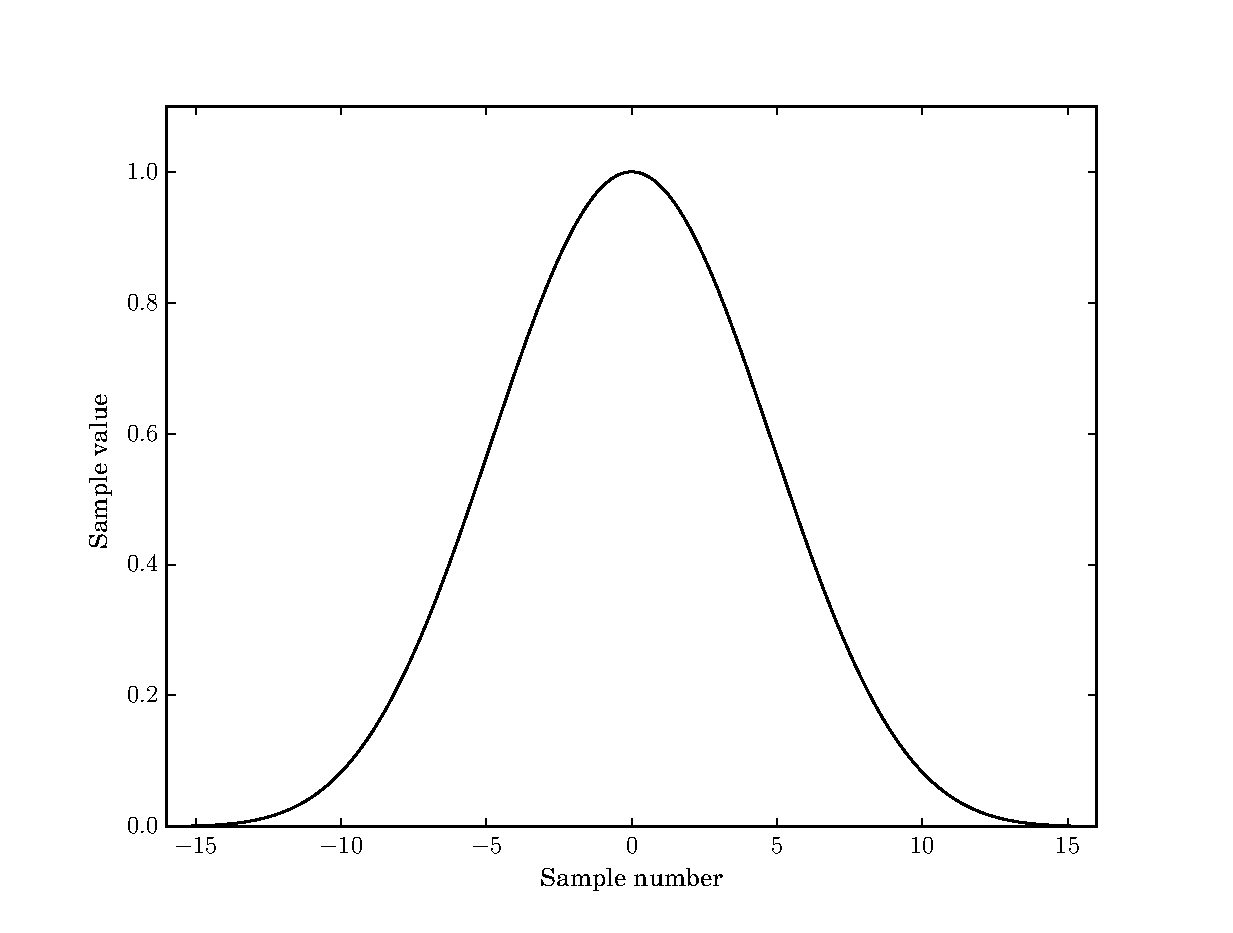
\includegraphics[width=\figwidthscale\textwidth]{plots/c1_blackman_td.eps}
    \CaptionWithTitle{%
        \input{plots/c1_blackman_td.txt}%
    }{}
\end{figure}

\begin{figure}[!t]
    \centering
    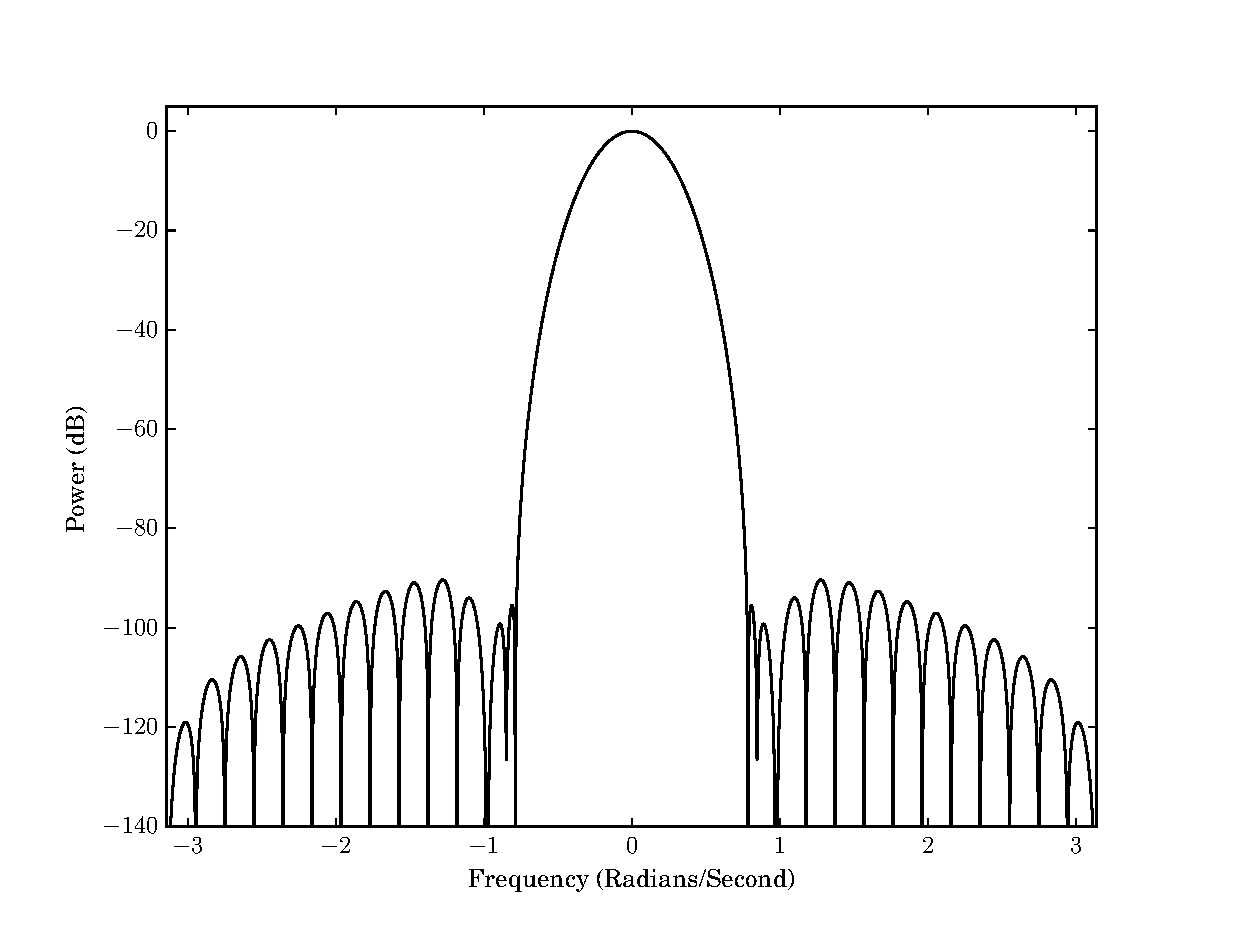
\includegraphics[width=\figwidthscale\textwidth]{plots/c1_blackman_fd.eps}
    \CaptionWithTitle{%
        \input{plots/c1_blackman_fd.txt}%
    }{}
\end{figure}

\begin{figure}[!t]
    \centering
    \includegraphics[width=\figwidthscale\textwidth]{plots/c1_vs_min_blackman_closeup.eps}
    \CaptionWithTitle{%
        \input{plots/c1_vs_min_blackman_closeup.txt}%
    }{\label{plot:c1vsminblackmancloseup}}
\end{figure}

\begin{table}
    \caption{\label{tab:optblackman}}
    \begin{center}
        \begin{tabular}{l c c c c }
            Window & $a_0$ & $a_1$ & $a_2$ & $a_3$ \\
            \hline
            Minimum & 0.35857 & 0.48829 & 0.14128 &
            0.01168 \\
            $\mathcal{C}^{1}$ & 0.35874 & 0.48831 &
            0.14127 & 0.01170
        \end{tabular}
    \end{center}
\end{table}

\begin{table}
    \caption{\label{tab:optvs4termblackman}}
    \begin{center}
        \begin{tabular}{l p{0.2\textwidth} p{0.2\textwidth} p{0.2\textwidth}}
            Window & Highest side-lobe level (dB) & 6-dB bandwidth in bins &
            Side-lobe fall-off (dB/octave) \\
            \hline
            Minimum & -92 & 2.72 & 6 \\
            $\mathcal{C}^{1}$ & -90 & 2.66 & 12 \\
        \end{tabular}
    \end{center}
\end{table}

As we are dealing with mixtures of sinusoids of small bandwidth, in addition to
the finite-time support constraint, we desire atoms whose inner-product is only
significant within a finite bandwidth of interest. To construct these atoms, we
multiply the Fourier atom by the window $w$
\[
    \psi_{\tau,\omega}^{\mathcal{F}_{w}}(n) = w(n-\tau) \exp(-j\omega(n-\tau))
\]

A good overview of different windows and their properties is given in
\cite{harris1978use}. We require that the window be at least
once-differentiable and zero outside of a certain interval, therefore, somewhat
informally, we require
\[
    \lim_{n \rightarrow T} \psi(n) = \psi(T) = 0
\]

\subsection{The Hann window}

The \textit{Hann} window possesses this property
\[
    w_{h}(n) = \begin{cases}
        0.5 + 0.5 \cos \left( \frac{n}{T}\pi \right) & -T \leq n \leq T \\
        0 & \text{otherwise}
    \end{cases}
\]

The Hann window is a member of a class of windows constructed by summing scaled
harmonically related cosine functions, subject to the constraint that the
scaling coefficients sum to 1 so that the window have a value of 1 at $n=0$.
Letting $T=N/2$, where $N$ is the length of the window
\[
    w(n) = \begin{cases}
        \sum_{m=0}^{M-1}a_{m}\cos \left( \frac{2\pi}{N}mn \right) & -\frac{N}{2} \leq n
        \leq \frac{N}{2} \\
        0 & \text{otherwise}
    \end{cases}
\]
With $M=2$ and $a_0 = a_1 = 0.5$, we have the Hann window.

The simple expression for its calculation and good trade-off between main-lobe
width and side-lobe height make the Hann window a popular choice in many signal
processing applications. The expression for its Fourier transform is such that
fast digital implementations of windowing a signal by a Hann window involve no
multiplies \cite[p.~183]{harris1978use}. A recursive implementation of the
DTSTFT is possible when windowing with the Hann window, which is important for
applications where little storage is available \cite[p.~102]{stankovic2014time}.
In spite of all its merits, other windows have been proposed that have superior
qualities, such as lower side-lobes.

\subsection{Continuous Blackman-Harris windows}

A family of windows with certain properties superior to the Hann window is the
\textit{Blackman-Harris} family of windows. These are also sum-of-cosine
windows. For these windows, optimization techniques were used to search for
coefficients giving minimum height of the highest side-lobe (maximum out-of-band
rejection) \cite{rabiner1970approach}. The 4-term window whose coefficients $a$
are listed in Table~\ref{tab:optblackman} has a maximum side-lobe level of 92
dB, just shy of the quantization noise of a 16-bit linear pulse code modulated
signal (96 dB). This window has a very large main-lobe which means two sinusoids of
similar frequency will be difficult to resolve. Furthermore, the window has a
discontinuity at its boundaries, e.g., $w \left( \frac{N}{2} \right) \neq 0$ and
is not once-differentiable. In any case the window is valuable in that it
effectively nulls any influence of signals outside of a bandwidth of interest.

It should be clarified that when we compare the widths of the main-lobes of two
windows, we compare two windows of the same length. Of course, the bandwidth of
a window can also be decreased by increasing its length, at the expense of
time-resolution. When searching for windows superior to the Hann window, we are
motivated by our ability to describe the signal with more detail between two
analysis frames than would be possible with a simple linear-phase sinusoid
model. Using a longer window to decrease the main-lobe width is not problematic
in this case, but we would still like a high level of signal rejection outside
of the bandwidth of interest for improved estimation accuracy of the signal
parameters. For this reason, we search for windows that have very low side-lobe
height and are also once-differentiable, without caring so much about the width
of the main-lobe. To find a window with properties similar to the 4-term
Blackman-Harris window but without a discontinuity, we solve the optimization
problem
\[
        \min||a-\tilde{a}||_2 \\
\]
subject to
\[
        w_{\tilde{a}} \left( \frac{N}{2} \right)
            = w_{\tilde{a}} \left( \frac{-N}{2} \right) = 0
\]
\[
        \sum_{m}^{M-1} a_{m} = 1
\]
where
\[
    w_{\tilde{a}}(n) = \begin{cases}
        \sum_{m=0}^{M-1}\tilde{a}_{m}\cos \left( \frac{2\pi}{N}mn \right) & -\frac{N}{2} \leq n
        \leq \frac{N}{2} \\
        0 & \text{otherwise}
    \end{cases}
\]
The solution $\tilde{a}^{\ast}$ is given in Table~\ref{tab:optblackman} and
plots are given in Figure~\ref{plot:opt_blackman}. This window will be referred
to as the $\mathcal{C}^{1}$ 4-Term Blackman-Harris window. Some figures of merit
for the two windows are compared in Table~\ref{tab:optvs4termblackman} in a similar
fashion to \cite{harris1978use}. We see
that the $\mathcal{C}^{1}$ 4-Term Blackman-Harris window is not too different
from the Minimum 4-term Blackman-Harris window, but has the additional
desirable property of differentiability everywhere in its domain. A comparison
of the windows's endpoints is presented in
Figure~\ref{plot:c1vsminblackmancloseup}.

\section{Conclusion}

In this chapter we have developed the rationale for adopting the sinusoidal
model when analysing musical signals. In turn we have presented some techniques
for estimating the parameters of these signals. Obviously these techniques only
work as well as their assumptions are true --- for the best results we should
use these techniques only on signals that indeed contain sinusoids. For the
signals considered in this thesis, we assume this to be true.

The techniques presented in this chapter are typically used to estimate the
parameters of short signals as we see in the use of window functions to limit
the time-frequency extent of our analysis. For the source separation problem we
are interested in larger sinusoidal objects --- partials --- whose global
properties are more readily classified. We could use a very large
analysis window and a high-order polynomial for phase when solving for the
coefficients, but the size of the linear system to be solved in
\ref{eq:ddmsyseq} will increase quadratically in the order of the model.
Furthermore, it is difficult to account for situations where the signal is
corrupted or briefly absent. In these situations we may prefer to use
interpolation to reconstruct the signal in the corrupted region. For these
reasons, we prefer to make multiple estimations of the parameters of low-order
models and connect those estimations thought of as belonging to a single
partial. We will see in Chapter~\ref{chap:exphsmodel} that this will allow
postulating a higher-order phase model. Before that is possible, however, we
must determine how to connect multiple estimations to form partials.
